\label{chapter:metodo}
\par
Este capítulo descreve o método proposto neste trabalho, baseado transformações de código para análise de circuitos lógicos descritos em VHDL utilizando 
\textit{Bounded Model Checking}, neste caso o \textit{model checker} ESBMC.

%======================
%Visão geral do método
%======================
\section{Visão geral do método}

\par
O método proposto consiste na tradução de um código em VHDL para linguagem e C e posteriormente a análise de deste programa, com base nas assertivas inseridas em um arquivo externo.  Inicialmente o código em VHDL é passado para ferramenta juntamente com outro arquivo contendo as variáveis de entrada, saída, pré-condições e pós-condições. Seguidamente é passado para duas ferramenta de tradução, inicialmente para Verilog que é instrumentado durante a execução e posteriormente traduzido para C. Após as traduções, as pré-condições e pós-condições, conforme o arquivo, são adicionadas ao códigos C e o mesmo é analisado pela ferramenta ESBMC. Caso alguma condição seja violada, o contra exemplo é apresentado ao usuário.

\begin{figure}[H]
	\begin{center}
    \caption{\label{fig:Fluxo_ferramenta}Ciclo da ferramenta}
	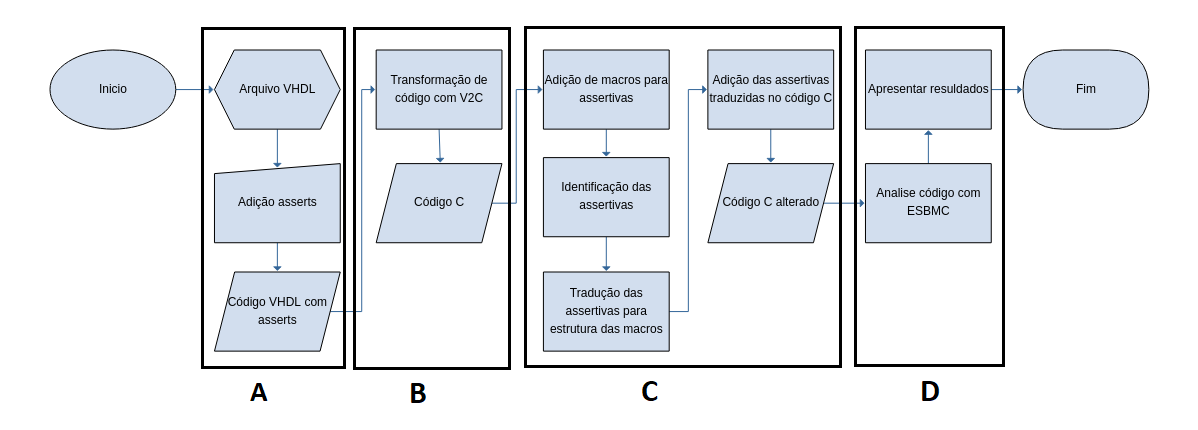
\includegraphics[scale=0.55]{Figuras/Fluxo_ferramenta.png}
	\end{center}
    \legend{Fonte: Própria}
\end{figure}

\par
Com o intuito de auxiliar nas explicações apresentadas nas próximas seções, o código na \autoref{fig:code_exemplo} será utilizado nas explanações, bem como será apresentado todas as alterações do mesmo, conforme cada etapa do método.  

\begin{figure}[H]
\caption{\label{fig:code_exemplo} Exemplo de código VHDL de ULA com portas AND e OR.}
	\begin{center}
    \begin{minipage}{0.7\textwidth}
    \begin{lstlisting}       
library ieee;
use ieee.std_logic_1164.all;

ENTITY Ula_tcc IS
PORT(A,B,Binvertido,Op1:IN std_logic;
	  Resultado:OUT std_logic);
END Ula_tcc;

ARCHITECTURE Ula_tcc_behavl OF Ula_tcc IS
SIGNAL and_port: std_logic;
SIGNAL or_port: std_logic;
SIGNAL mux2x1: std_logic;
BEGIN
	PROCESS(A,B,Binvertido,Op1)
	BEGIN
		IF(Binvertido = '0') THEN
			mux2x1 <= B;
		ELSE
			mux2x1 <= NOT B;
		END IF;
		and_port <= A AND mux2x1;
		or_port <= A OR mux2x1;
		IF(Op1 = '0') THEN
			Resultado <= and_port;
		ELSIF(Op1 = '1') THEN
			Resultado <= or_port;
		END IF;
	END PROCESS;
END Ula_tcc_behavl;
    \end{lstlisting}
    \end{minipage}
	\end{center}
    \legend{Fonte: Própria.}
\end{figure}

O código é um conceito básico de ula, formado apenas pelas portas AND e OR, além de um inversor o qual inverte o sinal de entrada, caso seja necessário. A saida deste inversor é ligado as portas AND e OR, e a saída destas porta é ligada a um multiplixador de duas entradas. Ao final, a saída do multiplixador será um dos sinais de entrada, ou seja, ou o sinal enviado pela porta AND ou pela porta OR e este sinal de saída será determinado de acordo com o sinal de escolha enviado ao multiplexador.

%========================
%Código VHDL e arquivo externo
%========================
\section{Código VHDL e arquivo externo}
\label{cap:vhdl_assertivas}

A primeira etapa do método consiste inicialmente no código VHDL a ser analisado, juntamente com o arquivo contendo as informações de entradas e saídas do código e também as pré-condições, que são condições que devem ser verdadeira antes da execução de um algum código ou trecho de código, e pós-condições que são condições declaradas e devem ser verdadeiras após a execução de um código ou trecho de código.

\par
O arquivo, \autoref{fig:arquivo_externo}, deve conter todas as variáveis de entrada e saída do código VHDL, apenas o nome da variável em ambos os casos. As variavéis de entrada são declaradas na linha \textbf{INPUT} e as variaveis de saída são declaradas na linha \textbf{OUTPUT}. Nas linhas seguintes são informadas as pré-condições e pós-condições que serão introduzidas ao código em etapas posteriores do processos.

\begin{figure}[H]
\caption{\label{fig:arquivo_externo} Exemplo de arquivo externo.}
	\begin{center}
    \begin{minipage}{0.8\textwidth}
    \begin{lstlisting}       
INPUT:A==1,B==1,Binvertido,Op1
OUTPUT:Resultado
PRECONDITION:
POSTCONDITION:Resultado==and_port||Resultado==or_port
    \end{lstlisting}
    \end{minipage}
	\end{center}
    \legend{Fonte: Própria.}
\end{figure}

\par
Em comparação ao método anterior, as diferenças consistem principalmente em as assertivas não estarem mais presentes diretamente no código VHDL, desta forma, o mesmo é utilizado apenas nas etapas de tradução. A principal vantagem é a não necessidade de elementos comentados ao código VHDL e com isso o código fica mais legível e também sem a necessidade de modificação ou inserção de trecho para funcionamento da ferramenta em questão.

%===================================
%Tradução de VHDL para C e instrumentações de código
%===================================
\section{\label{cap:traducao}Tradução de VHDL para C e instrumentações de código}

\par

A primeira etapa é a tradução de código entre VHDL para C, contudo, diferente do demonstrado no primeiro método, onde apenas uma única ferramenta realizava a tradução, nesta nova reformulação do método faz a utilização de duas ferramentas de tradução, inicialmente para Verilog e uma segunda ferramenta faz a tradução para C. Isso possibilita uma um aumento no potencial da tradução, contudo, devido ao uso de duas ferramentas, alguns erros ainda podem ser verificados na tradução.

\par
Devido ao uso das ferramentas, também é necessário mais uma etapa de instrumentação, sendo uma após a tradução para Verilog e outra após a tradução para C. A primeira instrumentação modifica o código para que segunda ferramenta de tradução possa executar a tradução corretamente e a segunda instrumentação adiciona as assertiva, de acordo com o introduzido no arquivo citado na seção anterior. Nas próximas subseções serão explicado com mais detalhes as traduções e as instrumentações

%================================================
%Tradução para Verilog e instrumentação de código
%================================================
\subsection{Tradução para Verilog e instrumentação de código}

\par
A primeira ferramenta de tradução utilizada, chamada VHD2Vl\cite{vhd2vl}, realiza a tradução do código VHDL para o código Verilog. O principal motivo de utilizar esta ferramenta deve-se a apresentar melhores resultados na tradução dos códigos, contudo, também apresenta alguma questões a serem observadas nas traduções. 

\par

Entre estas observações esta encontra-se a utilização das estrutura de std\_logic, std\_logic\_vector, integer e boolean. Também permite a utilização clock events das estruturas de controle, como if, elsif, else, case. A ferramenta também permite a instância de módulos no código VHDL, contudo o mesmo é ignorado na tradução o que causa erros de análise. Também é ignorado qualquer assertiva existente no código, tornando assim, mais necessário um arquivo externo com assertivas e condições a serem adicionadas ao texto\cite{vhd2vl}.


\begin{figure}[H]
\caption{\label{fig:codigo_verilog} Código da \autoref{fig:code_exemplo} traduzido pela ferramenta Vhd2vl.}
	\begin{center}
    \begin{minipage}{0.7\textwidth}
    \begin{lstlisting}
[...]
module Ula_tcc(
input wire A,
input wire B,
input wire Binvertido,
input wire Op1,
output reg Resultado
);

reg and_port;
reg or_port;
reg mux2x1;

  always @(A, B, Binvertido, Op1) begin
    if((Binvertido == 1'b0)) begin
      mux2x1 <= B;
    end
    else begin
      mux2x1 <=  ~B;
    end
    and_port <= A & mux2x1;
    or_port <= A | mux2x1;
    if((Op1 == 1'b0)) begin
      Resultado <= and_port;
    end
    else if((Op1 == 1'b1)) begin
      Resultado <= or_port;
    end
  end
endmodule
    \end{lstlisting}
    \end{minipage}
	\end{center}
    \legend{Fonte: Própria.}
\end{figure}

\par
Contudo, o código conforme apresentado acima, não pode ser traduzido para C, pois esta fora do padrão aceito pela ferramenta V2c, que realiza a tradução de verilog para C. Com isso é necessário uma instrumentação de código para que o mesmo possa ser traduzido. Esta intrumentação consiste na alteração dos modo de declaração das variavéis, na alteração de palavras chaves utilizadas no verilog e na busca de elementos que estejam dentro com escopo \textit{always@()}, que contém a arquitetura do código.

\begin{figure}[H]
\caption{\label{fig:codigo_verilog_declaracao} Diferença da declaração das variáveis após a intrumentação.}
	\begin{center}
    \begin{minipage}{0.7\textwidth}
    \begin{lstlisting}
[...]
module Ula_tcc(
input wire A,
input wire B,
input wire Binvertido,
input wire Op1,
output reg Resultado
);
[...]
    \end{lstlisting}
    \end{minipage}
    \legend{(a)}
    \begin{minipage}{0.7\textwidth}
    \begin{lstlisting}
module Ula_tcc(A,B,Binvertido,Op1,Resultado);
input wire A;
input wire B;
input wire Binvertido;
input wire Op1;
output Resultado;
reg Resultado;
[...]
    \end{lstlisting}
    \end{minipage}
    \legend{(b)}
	\end{center}
    \legend{Fonte: Própria.}
\end{figure}

\par
A primeira adaptação a ser feita é na declaração das variavéis. Conforme a \autoref{fig:codigo_verilog_declaracao}(a) apresenta a declaração após a a tradução e a \autoref{fig:codigo_verilog_declaracao}(b) apresenta após a instrumentação. As mudanças consistem em o nome das variáveis serem declaradas como uma especie de parametro e logo abaixo seus respectivos tipo, fora do modulo. Outra alteração é com relação ao \textbf{Output reg}, onde primeiro se declara como saida e depois como reg a mesma variavel, como apresentado na linha 7 e 8 da \autoref{fig:codigo_verilog_declaracao}(b) em relação a linha 7 da \autoref{fig:codigo_verilog_declaracao}(a).

\par
Outra alteração necessário é que nenhuma variavel seja declarada dentro do modulo Always@(), pois gera a não tradução do código por parte da ferramenta. Com isso toda e qualquer variavel que venha a ser utilizado durante a execução do código deve ser declarado antes do modulo always@(), conforme \autoref{fig:codigo_verilog_always}. E outra alteração consiste nas palavras reservadas, visto que verilog utiliza a palavra \textbf{define} para definição de constante. Esta alteração é importante, pois evita que o código seja traduzido de maneira errada.

\begin{figure}[H]
\caption{\label{fig:codigo_verilog_always} Declaração de variáveis anteriores ao modulo Always@()}
	\begin{center}
    \begin{minipage}{0.7\textwidth}
    \begin{lstlisting}
[...]
reg and_port;
reg or_port;
reg mux2x1;

always @(A, B, Binvertido, Op1) begin
    [...]
endmodule
    \end{lstlisting}
    \end{minipage}
	\end{center}
    \legend{Fonte: Própria.}
\end{figure}

\par

%================================================
%Tradução para Verilog e instrumentação de código
%================================================
\subsection{Tradução para C e adição das pre-condições e pós-condições.}

\par
A segunda parte da tradução é realizada pela ferramenta V2C \cite{mukherjee2016v2c}. Como citado anteriormente, após a instrumentação no código verilog o mesmo pode ser traduzido para C, conforme apresentado na \autoref{fig:codigo_C}. Após a tradução o código recebe as assertiva e inicializações de variáveis.

\par
Toda parte de arquitetura do código VHDL após a tradução para C é colocada em uma função de mesmo nome do arquivo. Também é definido uma \textit{struct} que contem as variavies que foram declaradas como \textit{output} e também variaveis que tenham sido declaradas para serem
utilizadas na execução da arquitetura, como os sinais por exemplo. As variaveis de entrada são declaradas na função main() e são repassadas como parametros da função.

\par
A necessidade desta \textit{struct} deve-se ao fato de que esta variáveis podem ter seus valores alterados em tempo de execução. Devido a este fato, variaveis são criadas para armazenar valores antigos e também receber novos valores, como ocorre nas linhas treze, catorze, quinze e desseseis da \autoref{fig:codigo_C}. Nota-se que estas variavéis possuem o mesmo nome das variaveis da \textit{struct}, com a adição do sufixo \_old.

\par
Após a etapa de conversão para linguagem C ocorre uma nova etapa de instrumentação de código, onde as assertivas serão introduzidas ao código C. Para isso faz-se necessário a utilização do arquivo de pre-condições e pos-condições passado para ferramenta juntamente com o código VHDL e apresentado na \autoref{fig:arquivo_externo}.

\begin{figure}[H]
\caption{\label{fig:codigo_C} Código C traduzido após a intrumentação no verilog.}
	\begin{center}
    \begin{minipage}{0.7\textwidth}
    \begin{lstlisting}
#include <stdio.h>
#include <assert.h>
#define TRUE 1
#define FALSE 0
struct state_elements_Ula_tcc{
_Bool Resultado;
_Bool and_port;
_Bool or_port;
_Bool mux2x1;
};
void Ula_tcc(_Bool A, _Bool B, _Bool Binvertido, _Bool Op1, _Bool *Resultado){
  struct state_elements_Ula_tcc  sUla_tcc;
  _Bool Resultado_old;
  _Bool and_port_old;
  _Bool or_port_old;
  _Bool mux2x1_old;
  mux2x1_old = sUla_tcc.mux2x1;
  and_port_old = sUla_tcc.and_port;
  or_port_old = sUla_tcc.or_port;
  Resultado_old = sUla_tcc.Resultado;
  if((unsigned char)Binvertido == 0){
    sUla_tcc.mux2x1 = B;
  }
  else{
    sUla_tcc.mux2x1 = !B;
  }
  sUla_tcc.and_port = A && mux2x1_old;
  sUla_tcc.or_port = A || mux2x1_old;
  if((unsigned char)Op1 == 0){
    sUla_tcc.Resultado = and_port_old;
  }
  else{
    if((unsigned char)Op1 == 1){
      sUla_tcc.Resultado = or_port_old;
    }
  }
}
void main() {
_Bool A;
_Bool B;
_Bool Binvertido;
_Bool Op1;
_Bool Resultado;
Ula_tcc(A, B, Binvertido, Op1, &Resultado);
}
    \end{lstlisting}
    \end{minipage}
	\end{center}
    \legend{Fonte: Própria.}
\end{figure}

\par
Para a instrumentação é necessário a utilização de funções próprias do analisador, neste caso o ESBMC \cite{esbmc} e estas funções são: \textbf{ESBMC\_assume()}, \textbf{\_\_VERIFIER\_nondet\_int()} e \textbf{\_\_VERIFIER\_nondet\_bool()}. A função \textbf{ESBMC\_assume()} permite que uma variável assuma um valor especifico. As funções \textbf{\_\_VERIFIER\_nondet\_int()} e \textbf{\_\_VERIFIER\_nondet\_bool()} modelam valores inteiros e booleanos não deterministicos respectivamente.

\par
A utilização da função ESBMC\_assume() é utilizada quando alguma variável foi inicializada no arquivo, desta forma a mesma é inicializada no código. Na linha 1 da \autoref{fig:arquivo_externo} é declarada variavel inicializada e nas linhas 49 e 50 da \autoref{fig:codigo_C_assert} é utilizado as função para declaração das variaveis. Desta forma o seta estes valores para aquela variavel no tempo de execução da analise.

\par
A importância das funções \textbf{\_\_VERIFIER\_nondet\_int()} e \textbf{\_\_VERIFIER\_nondet\_bool()} no desenvolvimento do método é evitar que um determinado estado do código não possa ser alcançado, devido a não inicialização de variáveis. Estas funções são utilizadas nas variaveis de entrada não inicializadas e as outras variaveis que não são inputs e nem outputs. Na \autoref{fig:codigo_C_assert}, linhas 14,15 e 16 apresenta o uso desta função.

\par
Em outras palavras, na instrumentação de código é realizado a adição das assertivas do modelo utilizado no arquivo para para o modelo utilizado em linguagem C, além como de outras funções que possam ser utilizados pelo VHDL. Ao final da instrumentação o código C fica disponível para que possa ser dado como entrada para outras ferramentas de verificação de código e não apenas o ESBMC.

\begin{figure}[H]
\caption{\label{fig:codigo_C_assert} Código C adição das assertivas.}
	\begin{center}
    \begin{minipage}{0.7\textwidth}
    \begin{lstlisting}
#include <stdio.h>
#include <assert.h>
#define TRUE 1
#define FALSE 0
struct state_elements_Ula_tcc{
_Bool Resultado;
_Bool and_port;
_Bool or_port;
_Bool mux2x1;
};
void Ula_tcc(_Bool A, _Bool B, _Bool Binvertido, _Bool Op1, _Bool *Resultado)
{
  struct state_elements_Ula_tcc  sUla_tcc;
  sUla_tcc.mux2x1 = __VERIFIER_nondet_bool();
  sUla_tcc.and_port = __VERIFIER_nondet_bool();
  sUla_tcc.or_port = __VERIFIER_nondet_bool();
  _Bool Resultado_old;
  _Bool and_port_old;
  _Bool or_port_old;
  _Bool mux2x1_old;
  mux2x1_old = sUla_tcc.mux2x1;
  and_port_old = sUla_tcc.and_port;
  or_port_old = sUla_tcc.or_port;
  Resultado_old = sUla_tcc.Resultado;
  if((unsigned char)Binvertido == 0){
    sUla_tcc.mux2x1 = B;
  }
  else{
    sUla_tcc.mux2x1 = !B;
  }
  sUla_tcc.and_port = A && mux2x1_old;
  sUla_tcc.or_port = A || mux2x1_old;
  if((unsigned char)Op1 == 0){
    sUla_tcc.Resultado = and_port_old;
  }
  else{
    if((unsigned char)Op1 == 1){
      sUla_tcc.Resultado = or_port_old;
    }
  }
  assert(sUla_tcc.Resultado == and_port_old||sUla_tcc.Resultado == or_port_old);
}
void main() {
_Bool A;
_Bool B;
_Bool Binvertido;
_Bool Op1;
_Bool Resultado;
ESBMC_ASSUME(A == 1);
ESBMC_ASSUME(B == 1);
Binvertido = __VERIFIER_nondet_bool();
Op1 = __VERIFIER_nondet_bool();
Ula_tcc(A, B, Binvertido, Op1, &Resultado);
}
    \end{lstlisting}
    \end{minipage}
	\end{center}
    \legend{Fonte: Própria.}
\end{figure}
%=============================================
%Verificação de assertvas usando model checker
%=============================================
\section{Verificação de assertivas usando \textit{Model Checker}}

\par
O \textit{model checker} adotado no desenvolvimento de método é o ESBMC~\cite{cordeiro2012smt} na versão $3.0.0$ e conforme explicado na Seção~\ref{cap:bounded}, esta ferramenta recebe como entrada um código C ou C$++$ e também utiliza solucionadores SMT para análise do programa.

\par
Para verificação pode ser utilizado dois métodos de analise, sendo eles o SMT e a indução-k. O SMT é o meio principal de verificação, juntamente com o mesmo é adicionado as seguintes opções, estas que o analisador trabalhe diretamente e unicamente com as assertivas, evitando que outros fatores possam ser analisado no código:
\begin{itemize}
    \item \texttt{$--$no-pointer-check:} para não realizar a checagem de ponteiros no código;
    \item \texttt{$--$no-div-by-zero-check:} para não realizar a checagem de divisões por zero no código; e
    \item \texttt{$--$no-bounds-check:} para não realizar a checagem de array bounds no código.
\end{itemize}

\par
A analise através da indução-k só será realizado caso o tempo de analise atrávez do SMT não chegue a alguma resposta num tempo especifico. No caso desta ferramenta o tempo utilizado foi de 5 min.

\par
Desta forma o ESBMC realiza apenas a checagem necessária dentro da assertiva, evitando que outros parâmetros sejam verificados, sem a devida necessidade do mesmo. Ao final de todos os desdobramentos é apresentado o resultado, sendo positiva (sem erros) ou negativa (com violação de propriedades), dependendo da assertiva e do código analisado. Este processo se repete até a lista de assertivas ser finalizada. Para o exemplo apresentado na \autoref{fig:code_exemplo} é exibido a violação da propriedade na \autoref{fig:resultado}, confirmando assim um erro na definição da porta lógica analisada.
